\begin{problem}[Munkres \S53, Ex.\,7(abcd)]
Let $G$ be a topological group with operation $\cdot$ and identity element
$x_0$. Let $\Omega(G,x_0)$ denote the set of all loops in $G$ based at
$x_0$. If $f,g\in\Omega(G,x_0)$, let us define a loop $f\otimes g$ by the
rule
\[
(f\otimes g)(s)=f(s)\cdot g(s).
\]
\begin{enumerate}[label=(\alph*)]
\item Show that this operation makes the set $\Omega(G,x_0)$ into a group.
\item Show that this operation induces a group operation $\otimes$ on
  $\pi_1(G,x_0)$.
\item Show that the two group operations $*$ and $\otimes$ on
  $\pi_1(G,x_0)$ are the same. [\emph{Hint:} Compute
  $(f*e_{x_0})\otimes(e_{x_0}*g)$.]
\item Show that $\pi_1(G,x_0)$ is Abelian.
\end{enumerate}
\end{problem}
\begin{proof}
For part (a) we need to show that the operation (0) $\otimes$ is associative,
(1) $\Omega(G,x_0)$ is closed under $\otimes$, (2) $\Omega(G,x_0)$ contains
an identity element $e$ and (3) for every $f\in\Omega(G,x_0)$ there
exists an element $\bar f\in\Omega(G,x_0)$ such that $f\otimes\bar f=\bar
f\otimes f=e$. We shall proceed in order: (0) Let
$f,g,h\in\Omega(G,x_0)$. Then $(f\otimes g)\otimes h=f\otimes(g\otimes f)$
since the multiplication $\cdot$ is associative in $G$, i.e., since given
$t\in I$ we have $(f(t)\cdot g(t))\cdot h(t)=f(t)\cdot (g(t)\cdot h(t))$,
in particular this holds for all $\in I$. (1) Let $f$ and $g$ be loops at
$x_0$ then $f\otimes g=f(s)\cdot g(s)$
\end{proof}
\newpage
\begin{problem}[(A)]
Prove Proposition F from the note on the Fundamental Group of the
Circle.
\end{problem}
\begin{proof}
Recall proposition F:
\begin{proposition*}[F]
\begin{enumerate}[label={\normalfont(\roman*)}]
\item $W$ takes the class of the path $f_n(s)=(\cos(2\pi ns),\sin(2\pi
  ns))$ to $n$ (and therefore $W$ is onto).
\item $W$ is one-to-one.
\item $W$ is a homomorphism.
\end{enumerate}
\end{proposition*}
(i) Now, recall that $W\colon\pi_1(S^1,x_0)\to\ZZ$ defined by
$W([f])\coloneqq w(f)$ where $w(f)=\tilde f(1)$ where $\tilde f\colon
I\to\RR$ is the lift of $f$, i.e. $p\circ \tilde f=f$. Now, let $f_n$ be a
path as above. Now, by Proposition C, since
\[
f_n(s)=(\cos(2\pi ns),\sin(2\pi ns))=(\cos(2\pi\tilde
f_n(s)),\sin(2\pi\tilde f_n(s)))
\]
and $\tilde f_n(0)=0=n\cdot 0$, by Proposition C, it follows that
$f_n(s)=ns$. Thus, $\tilde f(1)=n$.

(ii) Suppose $f_1,f_2\colon I\to S^1$ and $\tilde f_1(1)=\tilde f_2(1)$

(iii)
\end{proof}
\newpage
\begin{problem}[(B)]
Prove Lemma G from the note on the Fundamental Group of the Circle. (Hint:
one way to do this is to use the fact, which you don’t have to prove, that
if $\sim$ is the equivalence relation on $[a,a+1]$ which identifies $a$ and
$a+1$ then the restriction of $p$ induces a homeomorphism
$[a,a+1]/{\sim}\to S^1$.)
\end{problem}
\begin{proof}
Recall the statement of Lemma G:
\begin{lemma*}[G]
For each $a\in\RR$, the map
\[
p_a\colon(a,a+1)\longrightarrow S^1-p(a)
\]
given by $p_a(u)=p(u)$ is a homomorphism.
\end{lemma*}
We shall proceed by the hint.
\end{proof}
\newpage
\begin{problem}[(C)]
Show that for every point $x\in S^n$ the space $S^n-x$ is homeomorphic to
$\RR^n$. You may use the fact, shown in Step 1 of the proof of Theorem
59.3, that $S^n$ with the \emph{north pole} removed is homeomorphic to
$\RR^n$. (Hint: linear algebra.)
\end{problem}
\begin{proof}
\end{proof}
\newpage
\begin{problem}[(D)]
Show that every loop in $S^n$ which is not onto is path-homotopic to a
constant path. (Hint: use Problem C).
\end{problem}
\begin{proof}
\end{proof}
\newpage
\begin{problem}[(E)]
Let $X$ be a topological space and let $A\subset X$ be a deformation
retract. In the space $X/A$, the set $A$ is a point (because it is an
equivalence class). Show that this point is a deformation retract of
$X/A$. (Hint: use p.\,289 \# 9.)
\end{problem}
\begin{proof}
Let $H\colon X\times I\to X$ be a deformation retraction from $X$ to $A$,
that is, $H(0,x)=\id_X$ and $H(1,x)=r(x)$ where $r\colon X\to A$ is a
retraction of $X$ onto $A$ and $\iota\colon A\hookrightarrow X$ is
the inclusion of $A$ into $X$. Let $p\colon X\to X/A$ be a quotient
map. Now, we want to construct a deformation retraction $h\colon X/A\times
I\to X/A$ from the quotient $X/A$ to $*$, which we shall use to denote the
image of $A$ in $X/A$ under $p$, and what better candidate than the map
induced by $p\circ H\colon X\times I\to X/A$ on the quotient $X/A\times
I$ into $X/A$. Consider the map $(p,\id_I)\colon X\times I\to X/A\times
I$. This map is a quotient map by Problem 9.2 (Munkres \S46,
x.\,9). Moreover, the map $p\circ H$ preserves the equivalence relation on
$X/A\times I$ since for any two representatives $(x_1,t)$ and $(x_2,t)$ of
$[(x,t)]$ in $X/A\times I$, we have $H(x_1,t)=H(x_2,t)$ if $x\in X-A$ and
$H(x_1,t)=H_2(x_2,t)$ so $p(H(x_1,t))=p(H(x_2,t))$ and if $x_1,x_2\in
A$ then $H(x_1,t),H(x_2,t)\in A$ so $p(H(x_1,t))=p(H(x_2,t))$. Thus, by
Theorem Q.3 the map $h\colon X/A\times I\to X/A$ induced by $H$, i.e., the
map defined  by $h(x,t)\coloneqq[H(x,t)]$, is continuous and the diagram
\begin{center}
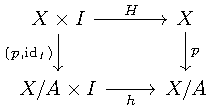
\includegraphics{figures/hw-11-def-retract}
\end{center}
commutes. We claim that $h$ is a deformation retraction from $X/A$ to
$*$. To that end, it suffices to show that $h(x,0)=\id_{X/A}$ and, using
suggestive notation, $h(x,1)=\bar r$ where $\bar r\colon X/A\to *$ is a
retraction of $X/A$ onto $A$ and $\bar\iota\colon *\hookrightarrow X/A$ is
the inclusion of $*$ into $X/A$. The first is easy to verify since
$h(x,0)=[H(x,0)]=[x]=\id_{X/A}$. Next, $h(x,1)=[H(x,1)]=[r(x)]$ and we
claim that $\bar r(x)\coloneqq [r(x)]$ is a retraction of $X/A$ into
$*$. The map $\bar r$ is continuous since $h$ is continuous (by Lemma 1
from Hw.\,\#9 Munkres \S18, Ex.\,11) and $\bar r\colon X/A\to *$ since
$r(x)\in A$ for every $x\in X$. It follows that $*$ is a deformation
retract of $X/A$.
\end{proof}

%%% Local Variables:
%%% mode: latex
%%% TeX-master: "../MA571-HW-Current"
%%% End:
